%%%%%%%%%%%%%%%%%%%%%%%%%%%%%%%%%%%%%%%%%%%%%%%%%%%%%%%%%%%%%%%%%%%%%%%%%
% This file is part of the LaTeX sources of the OMDoc 1.6 project descriptions
% Copyright (c) 2006 Till Mossakowski, Christian Maeder, Klaus L\"uttich
% This work is licensed by the Creative Commons Share-Alike license
% see http://creativecommons.org/licenses/by-sa/2.5/ for details
\svnInfo $Id: main.tex 8392 2009-06-17 04:21:23Z kohlhase $
\svnKeyword $HeadURL: https://svn.omdoc.org/repos/omdoc/trunk/doc/projects/hets/main.tex $
%%%%%%%%%%%%%%%%%%%%%%%%%%%%%%%%%%%%%%%%%%%%%%%%%%%%%%%%%%%%%%%%%%%%%%%%%

\begin{omgroup}[short=\hets,
   creators={mossakowski,maeder,luettich}]
   {\hets: The Heterogeneous Tool Set}

\ednote{project home page: \url{www.tzi.de/cofi/hets}}

\begin{omgroup}{Motivation}

\begin{quote}\sl\small
  ``There is a population explosion among the logical systems used in computer
  science. Examples include first order logic, equational logic, Horn clause logic, higher
  order logic, infinitary logic, dynamic logic, intuitionistic logic, order-sorted logic,
  and temporal logic; moreover, there is a tendency for each theorem prover to have its
  own idiosyncratic logical system. We introduce the concept of \emph{institution} to
  formalize the informal notion of `logical system'.''~\cite{GoguenBurstall92}
\end{quote}

In the area of formal specification and logics used in computer
science, numerous logics are in use:
\begin{itemize}
\item logics for specification of data types,
\item process calculi\twin{process}{calculus} and logics for the description of concurrent
  and reactive behaviour,
\item logics for specifying security requirements and policies,
\item logics for reasoning about space and time,
\item {\twintoo{description}{logic}s} for {\twintoo{knowledge}{base}s} in
  {\twintoo{artificial}{intelligence}} and for the {\twintoo{Semantic}{Web}},
\item logics capturing the control of name spaces and administrative domains (e.g.\ the
  ambient calculus), etc.
\end{itemize}

Indeed, at present, it is not imaginable that a combination of all these (and other)
logics would be feasible or even desirable --- even if it existed, the combined formalism
would lack manageability, if not become inconsistent. Often, even if a combined logic
exists, for efficiency reasons, it is desirable to single out sublogics and study
translations between these (cf.\ e.g.~\cite{Schneider04}).  Moreover, the occasional use
of a more complex formalism should not destroy the benefits of \emph{mainly} using a
simpler formalism.

This means that for the specification of large systems, heterogeneous multi-logic
specifications\twin{heterogeneous}{specification} are needed, since complex problems have
different aspects that are best specified in different logics.  Moreover, heterogeneous
specifications additionally have the benefit that different approaches being developed at
different sites can be related, i.e.\ there is a formal interoperability among languages
and tools.  In many cases, specialized languages and tools often have their strengths in
particular aspects. Using heterogeneous specification, these strengths can be combined
with comparably small effort.

{\omdoc} deliberately refrains from a full {\indextoo{formalization}} of mathematical
knowledge: it gains its flexibility through avoiding the specification of a formal
semantics of the logic(s) involved. By contrast, the Heterogeneous Tool Set
({\hets},~\cite{hets06}) is based on a rigorous formal semantics. {\hets} gains its
flexibility by providing \emph{formal interoperability}, i.e. integration of different
formalisms on a clear semantic basis.  Hence, {\hets} is a both flexible, multi-lateral
\emph{and} formal (i.e.\ based on a mathematical semantics) integration tool. Unlike other
tools, it treats logic translations (e.g.\ codings between logics) as first-class
citizens.
\end{omgroup}

\begin{omgroup}{Institutions, Entailment Systems and Logics}

Heterogeneous specification is based on individual (homogeneous) logics and
{\twintoo{logic}{translation}s}~\cite{MossakowskiHabil}. To be definite, the terms `logic'
and `logic translation' need to be formalized in a precise mathematical sense.  We here
use the notions of {\emph{\indextoo{institution}}}~\cite{GoguenBurstall92} and
{\emph{\twintoo{entailment}{system}}}~\cite{Meseguer89}, and of
{\emph{\indextoo{comorphism}}}~\cite{GoguenRosu02} between these.

Logical theories are usually formulated over some (user-defined)
vocabulary, hence it is assumed that an institution provides a notion
of \emph{signature}. Especially for modular specification, it is
important to be able to relate signatures, which is done by
\emph{signature morphisms}.  These can be composed, and hence form a
\emph{category of signatures and signature morphisms}.

Furthermore, an institution provides notions of \emph{sentences} and
\emph{models} (over a given signature $\Sigma$).  Models and sentences
are related by a \emph{satisfaction relation}, which determines when a
given sentence holds in a model.  An entailment system also provides
an \emph{entailment (provability) relation}, which allows to infer
sentences (conclusions) from given sets of sentences (premises, or axioms).

Finally, it is assumed that each signature morphism leads to
translations of sentences and models that preserve satisfaction and
entailment.

A {\emph{institution comorphism}} is a translation between two institutions.  It maps
signatures to signatures, sentences to sentences and models to models, such that
satisfaction is preserved (where models are mapped contravariantly, i.e.\ against the
direction of the comorphism).
  
We refer the reader to the literature~\cite{GoguenBurstall92,Meseguer89,MossakowskiEA05c}
for formal details of institutions and comorphisms. Subsequently, we use the terms
``institution'' and ``logic'' interchangeably, as well as the terms ``institution
comorphism'' and ``logic translation''.
\end{omgroup}

\begin{omgroup}{The Architecture of the Hets System}

\begin{figure}[ht]
  \begin{center}
    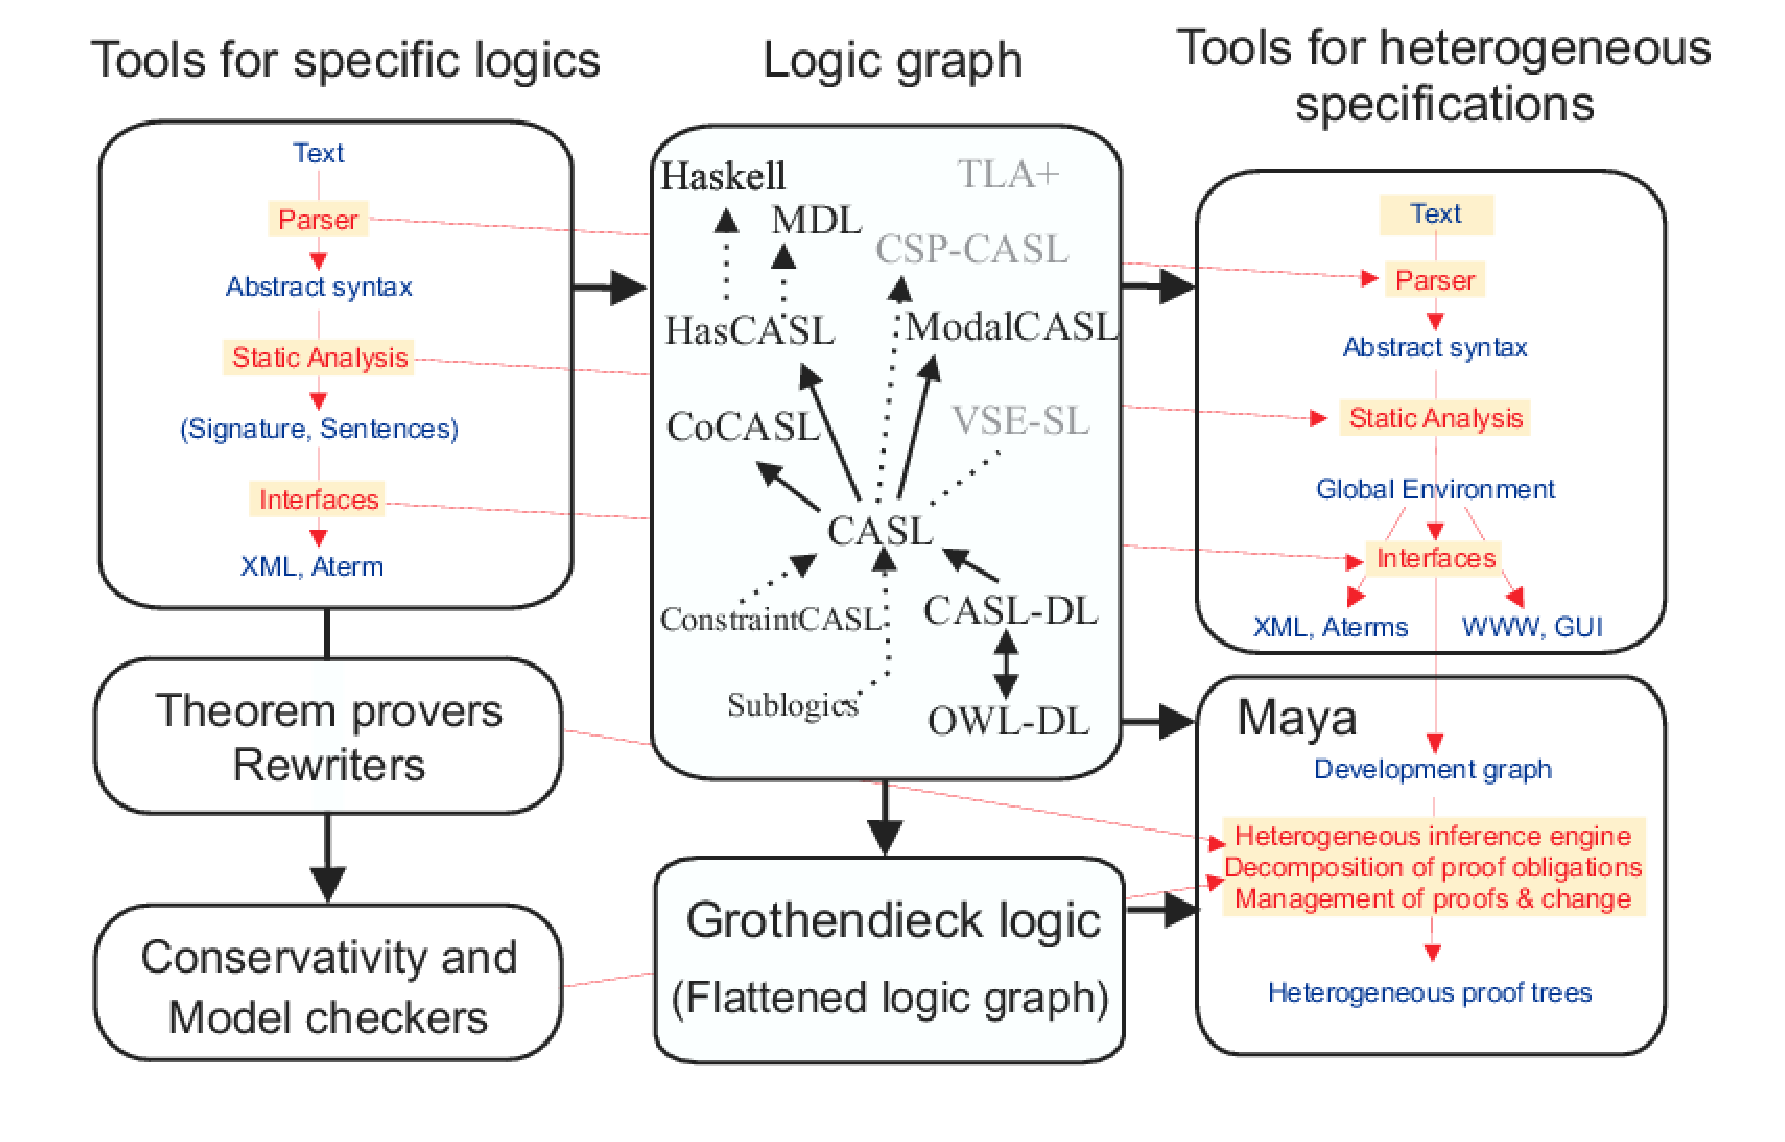
\includegraphics[width=\textwidth]{\projectsPath{hets/hets-new}}
    \caption{Architecture of the heterogeneous tool set}
    \label{fig:hetcats}
  \end{center}
\end{figure}

{\hets} is a tool for parsing, static analysis and proof management combining various such
tools for individual specification languages, thus providing a tool for heterogeneous
multi-logic specification (see Fig.~\ref{fig:hetcats}). The graph of currently supported
logics and logic translations is shown in Fig.~\ref{fig:LogicGraph}. However, syntax and
semantics of heterogeneous specifications as well as their implementation in {\hets} is
parametrized over an arbitrary such logic graph. Indeed, the {\hets} modules implementing
the logic graph can be compiled independently of the {\hets} modules implementing
heterogeneous specification, and this separation of concerns is essential to keep the tool
manageable from a software engineering point of view.

\begin{figure}
  \begin{center}
    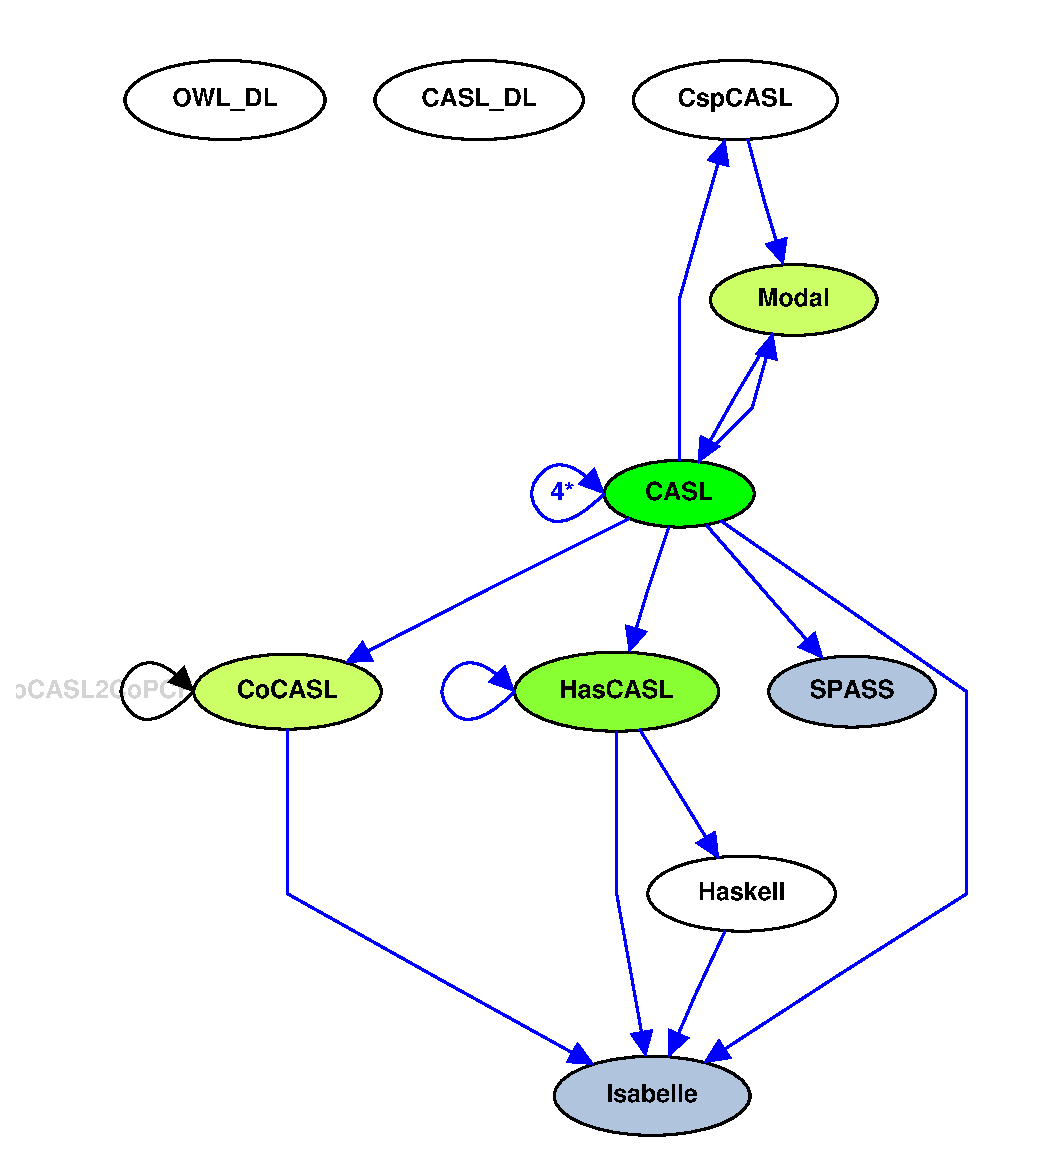
\includegraphics[scale=0.4]{\projectsPath{hets/LogicGraph}}
  \end{center}
  \caption{Graph of logics currently supported by {\hets}. The more an ellipse is filled,
    the more stable is the implementation of the logic.}
  \label{fig:LogicGraph}
\end{figure}

Heterogeneous {\casl} ({\hetcasl}; see~\cite{Mossakowski04}) includes the structuring
constructs of {\casl}, such as union and translation.  A key feature of {\casl} is that
syntax and semantics of these constructs are formulated over an arbitrary institution
(i.e.\ also for institutions that are possibly completely different from first-order logic
resp.\ the {\casl} institution). {\hetcasl} extends this with constructs for the
translation of specifications along logic translations.


Like {\maya} (see~\sref{maya}), {\hets} provides a representation of structured
specifications which are the logical basis for the {\emph{Complex theories}} and
{\emph{Development graphs}} of {\omdoc}\footnote{These are the modules {\CTHmodule{spec}}
  and {\DGmodule{spec}}, respectively.}.

For proof management, {\maya}'s calculus of development graphs has been extended with
hiding and adapted to heterogeneous specification. Development graphs provide an overview
of the (heterogeneous) specification module hierarchy and the current proof state, and
thus may be used for monitoring the overall correctness of a heterogeneous development.


{\hets} also provides a translation of {\casl} to and from a subset of
{\omdoc} (namely some formal first-order subset).  Future work aims at
a deeper integration of {\hets} and {\omdoc} that provides a
translation to and from {\omdoc} for each of the logics integrated in
{\hets}. Moreover, {\omdoc} itself will become a ``logic'' (but only
with syntax, without model theory) within {\hets}, such that also
informal {\omdoc} documents (or formal {\omdoc} documents written in a
logic currently not available in {\hets}) will be manageable for
{\hets}. In this way, the data formats of {\omdoc} and {\hets} will
converge, such that tools e.g.\ for searching, versioning or
management of change can be implemented uniformly for both.
\end{omgroup}
\end{omgroup}
%%% Local Variables: 
%%% mode: latex
%%% TeX-master: "../main"
%%% End: 

% LocalWords:  Hets hets Mossakowski Maeder uttich sublogics multi maya hets
% LocalWords:  hets
